\section{Introduction}
\label{sec:intro}

Richard Feynman's pitch for quantum computers was that nature is quantum, so simulating it efficiently
needs a machine that is itself quantum~\cite{feynman1982}. Fault-tolerant resource estimates now exist
for molecular energies and reaction paths~\cite{lee2021femoco,vonburg2021}. What is missing is a map of
where the boundary lies between ``classical computers are fine'' and ``a quantum machine is needed'' for
\emph{dynamics}. Resource estimates usually compare one classical method with one quantum algorithm and take
the inputs, above all the entanglement of the simulated state, as assumptions rather than measurements.

We study perhaps the simplest many-body process that is also chemically meaningful: real-time
tunneling in a small cluster. Put a few light particles in a trap with two valleys. A particle in the left
valley cannot climb the hill between them, but it can tunnel through it. When several particles interact,
the cluster as a whole switches coherently between two arrangements (which valley holds how many
particles), like a pendulum. This oscillation is the real-time signature of tunneling and what a simulator
has to reproduce. Coherent tunneling between equivalent structures is resolved spectroscopically in real
clusters, for example in the water hexamer prism~\cite{richardson2016}.

Four standard routes exist. \emph{Exact propagation} stores the wave function on a real-space
grid~\cite{kosloff1983,light2000} and diagonalizes or time-evolves it~\cite{lanczos1950,weisse2008,almohy2011}.
\emph{Tensor networks} store only the entanglement across cuts~\cite{white1992,vidal2004,schollwock2011,paeckel2019};
in chemical dynamics the multiconfiguration time-dependent Hartree method plays a similar
role~\cite{beck2000,wang2003}. \emph{Monte Carlo} samples paths~\cite{anderson1975,ceperley1980,sindzingre1989,richardson2011}
but meets a sign problem in real time~\cite{troyer2005,muhlbacher2008}. A \emph{quantum computer} stores the state in
qubits and evolves it with product-formula or qubitization
circuits~\cite{zalka1998,lloyd1996,kassal2008,childs2021trotter,low2019qubitization}. Each route is limited by a
different resource (memory, entanglement, variance, gate count), and the map of this paper is built by bounding
that resource for each of them. Our question is not whether a quantum computer can simulate tunneling, which it can in
principle~\cite{lloyd1996,buluta2009,georgescu2014}, but a sharper one:

\begin{quote}
\emph{For which particle masses and cluster sizes is real-time tunneling (a) beyond every classical route we can
afford, yet (b) affordable on a fault-tolerant quantum computer we can plausibly build?}
\end{quote}

\paragraph{The window as the bounds give it.}
Heavier particles tunnel more slowly, so the simulation must run longer and the quantum gate count
grows as $e^{2\mut/3}$; this sets an upper edge in $\mut$ that is logarithmic in the budget. Larger clusters make
every classical route more expensive; this sets a lower edge in $N$. In between lies a window (Fig.~\ref{fig:regime}).
The upper edge is an explicit function we can evaluate for one evolution. The lower edge is not: full-state storage is arithmetic, but tensor networks depend on how fast the entanglement of the state grows with $N$, and that
has to be measured. Measuring it is the main simulation work of this report.

\begin{figure}[t]
\centering
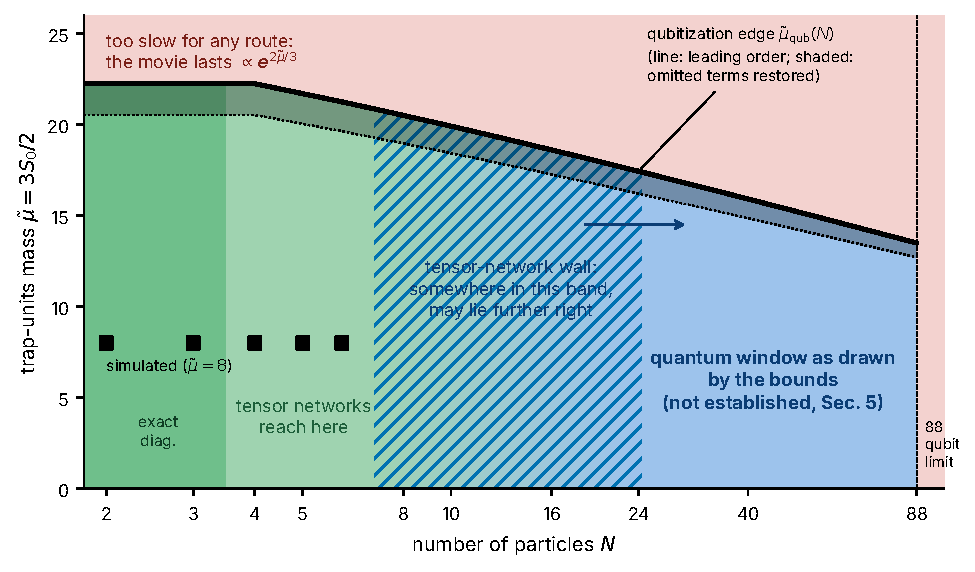
\includegraphics[width=0.8\textwidth]{figures/fig_regime.pdf}
\caption{\textbf{The window as the cost models draw it (and why it should not be read as a result about the dynamics).} Cluster size $N$
against the trap-units mass $\mut=3S_0/2$ (the tunneling time grows as $e^{2\mut/3}$). The curve is the qubitization edge of the leading-order cost model of \emph{one evolution}; the grey
band below it shows where the edge moves when two omitted terms are restored. Exact diagonalization (dark green) fails by an exact count (Table~\ref{tab:walls}). The tensor-network wall (hatched, fading) lies
in the band that the three entropy-growth scenarios of Section~\ref{sec:larger} give: first failing $N=\num{wall_pess_grid}$--\num{wall_opt_grid} when the bond
dimension is charged as $2^{S}$, and $N=\num{wallchi_sat_grid}$ when the measured Schmidt rank is charged instead (Section~\ref{sec:walls}). It may lie further
right, because the entropy is measured only up to $N=\num{Nmax_measured}$; it prices the entanglement of the prepared state, most of which is present without tunneling
(Section~\ref{sec:static}). Squares: the points simulated at $\mut=8$. The label \emph{quantum window} marks where the cost models leave a gap; this report does not establish it. \textbf{Imaginary-time Monte Carlo is not drawn and is not excluded:} it is sign-free in this model and is the nearest classical rival; it could close part of the window (Section~\ref{sec:mc}).
Budgets: Table~\ref{tab:params}.}
\label{fig:regime}
\end{figure}

\paragraph{What is, and is not, hard.}
Two nearby settings are easy classically, and we do not claim otherwise. If a single light particle tunnels through a
heavy, static background, the background acts as a fixed potential (Born--Oppenheimer~\cite{bornoppenheimer1927}), the
problem is one-body, and its cost per time step does not grow with the size of the background. If the background
reacts only locally and the entanglement stays low, a matrix product state with small bond dimension
suffices~\cite{vidal2004,schollwock2011,schuch2008}. Neither applies to the cluster studied here: all $N$ particles have
the same mass and any of them can cross, so there is no timescale gap; the pair interaction acts between every pair that
shares a valley, so there is no short chain of neighbours; and the entanglement generated by real-time dynamics is not
bounded in advance~\cite{calabrese2005}. We therefore measure it (Section~\ref{sec:measured}) and read the
tensor-network wall off the measured growth. Nothing here is a hardness theorem.

\paragraph{What this report is.}
The report is a bounds-first answer to this question and ends as a negative result: the window of Fig.~\ref{fig:regime} is what the bounds draw, and it is not established as a statement about the dynamics. The bounds and the measurements stand
(Sections~\ref{sec:measured} and~\ref{sec:discussion}); what does not stand is the reading that they open a window for the dynamics.
We therefore looked at what the prepared state is made of, by computing the eigenlevels of the Hamiltonian and the weight of the
start on each (Section~\ref{sec:static}). For $N\le5$ the state is two eigenstates plus a dressing, most of its entanglement
is static, and, if that persists, the signal is a short sum of cosines of quantities that do not involve time. The tensor-network walls price that static entanglement; they do not show that the dynamics is hard. Section~\ref{sec:open} states what remains.

\subsection{Parameters and conventions}
\label{sec:params}

Every choice that enters the results is listed in Table~\ref{tab:params}; the model itself is defined in
Section~\ref{sec:model}. Particles are distinguishable (labelled, like different isotopes), which is the worst case for the
classical side. Entropies are von Neumann entropies in bits. $\hbar=m=1$ in the simulations; $\mut$ is changed by
rescaling, never by changing the trap.

\begin{table}[ht]
\centering
\footnotesize
\caption{Parameters of the model, of the numerical representations and of the budgets. All values are read from the single configuration file of the simulations. The trap, the interaction and the budgets are choices, not fits; Appendix~\ref{app:choice} says why these values were chosen and Appendix~\ref{app:numerics} what each numerical setting controls.}
\label{tab:params}
\begin{tabular}{L{2.4cm}L{7.4cm}L{4.4cm}}
\toprule
Group & Quantity & Value \\
\midrule
Trap & barrier strength $A$, $U=A(x^2-1)^2+\tfrac12\omega_y^2y^2$ & $8$ \\
 & transverse $\omega_y^2$ & $2$ \\
Pair potential & Lennard-Jones $\epsilon$, $\sigma$, cap $V_{\rm cap}$ & $2$, $0.18$, $100$ \\
Particles & tilt $c+c_i$, offsets $c_i=(i-1)C_0$, $C_0$ & $0.15$; $c$ at resonance \\
 & mass, $\hbar$ (simulation units) & $1$, $1$ \\
Grid (basis 1) & cells $n_x\times n_y$, $M$; $\Delta x$, $\Delta y$ & $40\times30$, $1200$; $0.125$, $0.200$ \\
Modes (basis 2) & modes per particle $k$ (local dimension $d$) & $12$, $16$, $20$ \\
Qubits (basis 3) & qubits per particle $n_p$; auxiliary & $11$; $30$ \\
Starts & correlated: penalty $W$ on the wrong side & $30$ \\
Dynamics & Chebyshev propagation; window $T$; snapshot spacing $\Delta t$ (one protocol for all $N$) & $200$; $1.0$ ($201$ snapshots) \\
Working point & trap-units mass $\mut_0$; action $S_0$; switching time $t_0$ & $8$; $5.33$; $16.5$ \\
Budgets & memory $\Bmem$; compute $\Bflop$ & $\ensuremath{10^{12}}$ B; $\ensuremath{10^{20}}$ operations \\
 & logical qubits $\BQ$; T-gates $\BT$; precision $\varepsilon$ & $1000$; $\ensuremath{10^{12}}$; $\ensuremath{10^{-3}}$ \\
Cost models & Krylov vectors $v$; sweeps (compute prefactor $A_{\rm sw}$) & $10$; $100$ ($200$) \\
\bottomrule
\end{tabular}
\end{table}


\subsection{Findings in brief}
\label{sec:findings}

\begin{enumerate}[itemsep=0.2em]
\item \textbf{Exact methods and Monte Carlo.} Full-state storage is exponential in $N$ \stE{}. Real-time path sampling suffers the sign problem; imaginary-time Monte Carlo is sign-free in this model, is not excluded and is the nearest classical rival (Section~\ref{sec:mc}).
\item \textbf{Tensor networks.} Every layout pays $\chi\ge2^{S}$ for the entropy of a balanced cut \stE{}. The central-cut entropy was measured for
  $N=2$--\num{Nmax_measured} and grows by less per added particle than pair counting predicts (Fig.~\ref{fig:entropy}). A correlation graph reproduces the entropy of every subset to
  within \num{graph_maxdev} bit and picks the best layout \stM{}. Its pair weights fall roughly as $1/(N-1)$, as if the one-particle entropy were shared among the partners; this is
  a description of $N\le6$, not a derivation (Section~\ref{sec:graph}).
\item \textbf{Quantum route.} A leading-order qubitization count for \emph{one evolution} fits the budgets with room to spare and gives a mass edge that falls slowly with $N$ \stM{} (Section~\ref{sec:quantum}).
\item \textbf{The start is two levels plus a dressing} (Fig.~\ref{fig:spectrum}). For $N\le5$ the correlated start sits on two eigenstates (all particles in the crowded valley; one particle moved), with
  weight $B_2$ that falls with $N$ at fixed basis and rises with the basis size (Table~\ref{tab:static}, Fig.~\ref{fig:dressing}a). The rest lies within a few $J$ of the pair
  (Fig.~\ref{fig:dressing}b). An exact reflection symmetry removes the other levels (Fig.~\ref{fig:parity}).
\item \textbf{Most of the entropy is static.} Away from resonance, with no tunneling, the central entropy at $N=5$ is \num{off_Snat} bit against \num{Snat_N5} bit on resonance (Section~\ref{sec:static}).
  The tensor-network walls of Section~\ref{sec:walls} therefore price the isomers, not the transfer.
\item \textbf{A conditional reduction and an open question.} If the start stays in the span of the two states and a few sidebands, the signal is a sum of at most $(M+2)(M+3)/2$ cosines of static
  quantities, and the bond dimension is at most $(M+2)\chi_0$ (Proposition~\ref{prop:cond}). Whether $M(N)$ stays small is open; at fixed trap depth the regime itself ends near $N\approx\num{fu_Ntop_lo}$--\num{fu_Ntop_hi}
  (Fig.~\ref{fig:tilt}).
\item \textbf{The window} is therefore not established as a statement about the dynamics. It remains a statement about the price of one evolution on one side and of the static entanglement on the other.
\end{enumerate}

\paragraph{Status of statements.} \stE{} marks an identity or count; \stM{} a result derived under a stated model or measured with stated
parameters; \stC{} a result true if a named growth hypothesis holds. Section~\ref{sec:open} lists what is open. Appendix~\ref{app:choice} explains the choice of the model parameters, Appendix~\ref{app:proofs} holds the proofs,
Appendix~\ref{app:numerics} the numerical details and the raw logs behind each figure, Appendix~\ref{app:static} the spectrum of the start (method, one table of all cases, structural checks), and Appendix~\ref{app:quantum} the quantum cost model.
